\section{Literature Review}
\title{”TOWARDS BENCHMARK DATASETS FOR MACHINE LEARNING BASED WEBSITE PHISHING DETECTION: AN EXPERIMENTAL STUDY”}\\
Link: {\small \url{https://arxiv.org/pdf/2010.12847.pdf}}
\subsection{Objective}
To propose and experiment a general scheme for building reproducible and extensible datasets for website phishing detection, and to evaluate the performance of different machine learning techniques and features on the built dataset.
\subsection{Methodology}
URLs are collected from various sources and preprocessed, from which 87 features are extracted under different classes(URL, Content, External). The dataset is then balanced and shuffled. Two metrics are used for performance Evaluation, Accuracy and Macro F1 Score.\\
\begin{figure}[ht!]
    \centering
    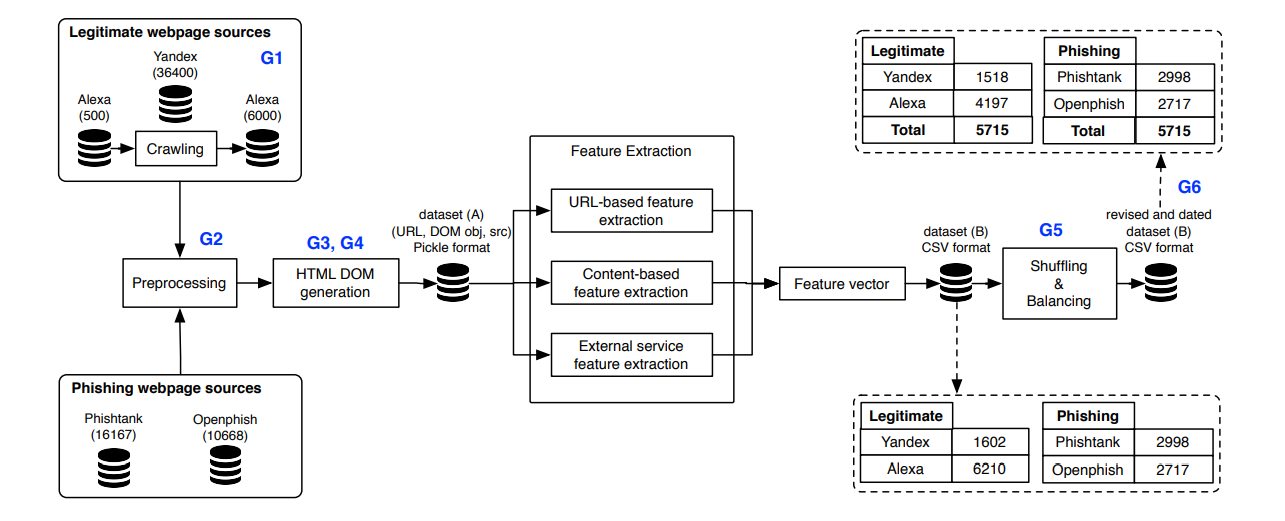
\includegraphics[width = 0.45\textwidth]{./images/data_prep.png}
    \caption{Dataset Preparation}
    \label{fig:1}
\end{figure}\\
The classifiers used are:
\begin{itemize}
    \item[-] Naive Bayes
    \item[-] Support Vector Model
    \item[-] Logistic Regression
    \item[-] Decision Tree
    \item[-] Random Forest
\end{itemize}
The following experiments were done:
\begin{itemize}
    \item[-] Best model for single or combination of feature classes
    \item[-] Combination of different models
    \item[-] Feature selection
    \item[-] Feature extraction runtime analysis
\end{itemize}
\subsection{Results}
A scheme for constructing benchmark datasets that canenable comparison, replication, and extension of website phishing detection systems was presented.\\
Random Forest was found to give the best accuracy for all the classes of features. External-based features provide the best accuracy, followed by URL-based and then Contentbased. Using hybrid features was found to be better than
using single class of features.\\
It was found that chi-square filter gave the best accuracy with less number of features and that filter ranking together with incremental removal of less important features improved the performance. Wrapper methods failed to improve the accuracy compared with filter methods and using ’Boruta algorithm’ was much faster than ’WrapperSubsetEval’.\\
Extraction time of different features and feature classes was investigated. It was found that content-based features were the most time consuming and that some hyperlinkbased features also caused severe network delays.
